\begin{quote}
  This chapter explores an approach to scene understanding that
  relates low--level image information directly to high--level
  variables describing scene categories and coarse geometry. We
  build on a well--known texture analysis approach in which pixels are
  identified with characteristic texture units known as
  textons. Extending previous work in texture analysis and image
  recognition, we show that this approach --- which has previously been
  applied to recognition of uniform textures --- extends to 
  high--level scene understanding problem in which the input image is
  composed of many objects and surfaces. We propose a novel
  recognition model in which we measure the displacement between
  texton occurrences in an image rather than their absolute location
  or overall frequency. We apply our ideas to two classification
  tasks: place recognition and camera orientation
  classification. Comparisons with the gist descriptor of Torralba
  \etal show superior performance on both tasks.\footnotemark
\end{quote}

\footnotetext{This work was published in part in:

{ \setlength{\parindent}{0pt} 
  \textit{Flint, Murray, and Reid,} ``Learning Textons For
  Real--Time Scene Context'', in \textit{Proceedings of the
    First International Workshop on Ego--Centric Vision, 2009}\cite{Flint09}
} 
}

\section{Introduction}
One important aspect of scene understanding is the ability to
differentiate between logical areas within an environment, such as
rooms in a house. This problem is important in the domain of augmented
reality because knowledge of the location of a user will give a strong
indication as to the activities the user might undertake and the
objects with which they are likely to interact. 

Outside this specific application area, place recognition can be used
as a generic source of context for further scene understanding
tasks. Object recognition, semantic segmentation, and semantic
reconstruction are all likely to benefit from a prior on place
categories, since such information would correlate well with the
location of objects, the function of surfaces, and the geometric
structure of the environment.

The place recognition problem we propose in this chapter associates
many images of a logical region --- rooms within a house in our case
--- with a single place category. This means that there may be image
pairs observing no common 3D locations, yet are associated with the
same category, and hence the system will be expected to recognise them
as associated with the same logical place. We also tackle the problem
of identifying the approximate tilt of the camera from a single
image. This problem requires the categorisation of images into 3
categories: ``upwards--facing'', ``downward-facing'', and
``straight-facing''.

We pursue an approach motivated by the texton model developed by
Julesz \cite{Julesz81} and introduced to the computer vision community
somewhat later \cite{Zhu02}. We show that low--level texture elements
can be related to the high--level variables of interest to us, and
that doing so yields state--of--the--art results for both scene
understanding problems.

The remainder of this chapter is organised as follows. First we
introduce the notion of textons, which form the basis of our
approach. Next we motivate the use of textons for scene understanding
problems in general by exploring the relationship between textons and
scenes. We then describe our probabilistic model relating textons to
place recognition and camera classification in detail. Next we present
an empirical comparison between our system and the gist descriptor of
Torralba \etal, followed by discussion and concluding remarks.

\section{Background}
\label{sec:background}
The notion of textons as atomic texture elements was born in the
neuroscience community when in 1981 Julesz \cite{Julesz81} introduced
textons as part of his theory of human visual attention. Julesz
defined textons as elongated blobs, line terminators, and line
intersections. Several researchers have proposed definitions of
textons for use in computer vision applications (see \cite{Zhu02} for
an extensive discussion), including both topological and statistical
descriptions. We follow the statistical account first proposed by
Malik \etal \cite{Malik99}. Under this definition, an image is passed
through a filter bank, producing a set of response images. Each pixel
is then associated with a feature vector that contains each filter's
response for that pixel. The feature vectors are then clustered and
the resultant cluster centres become the texton exemplars.

At evaluation time the input images are passed through the same set of
filters, and each pixel is again associated with a feature vector
containing the filter responses at that point. Next, each pixel is
labelled according to the index of the texton exemplar (from the
training phase) closest to it in the L2 sense. The image is
henceforth represented as an array of texton indices (the ``texton
map''); the remainder of the image data is discarded.

\begin{figure}[htp]
  \centering
  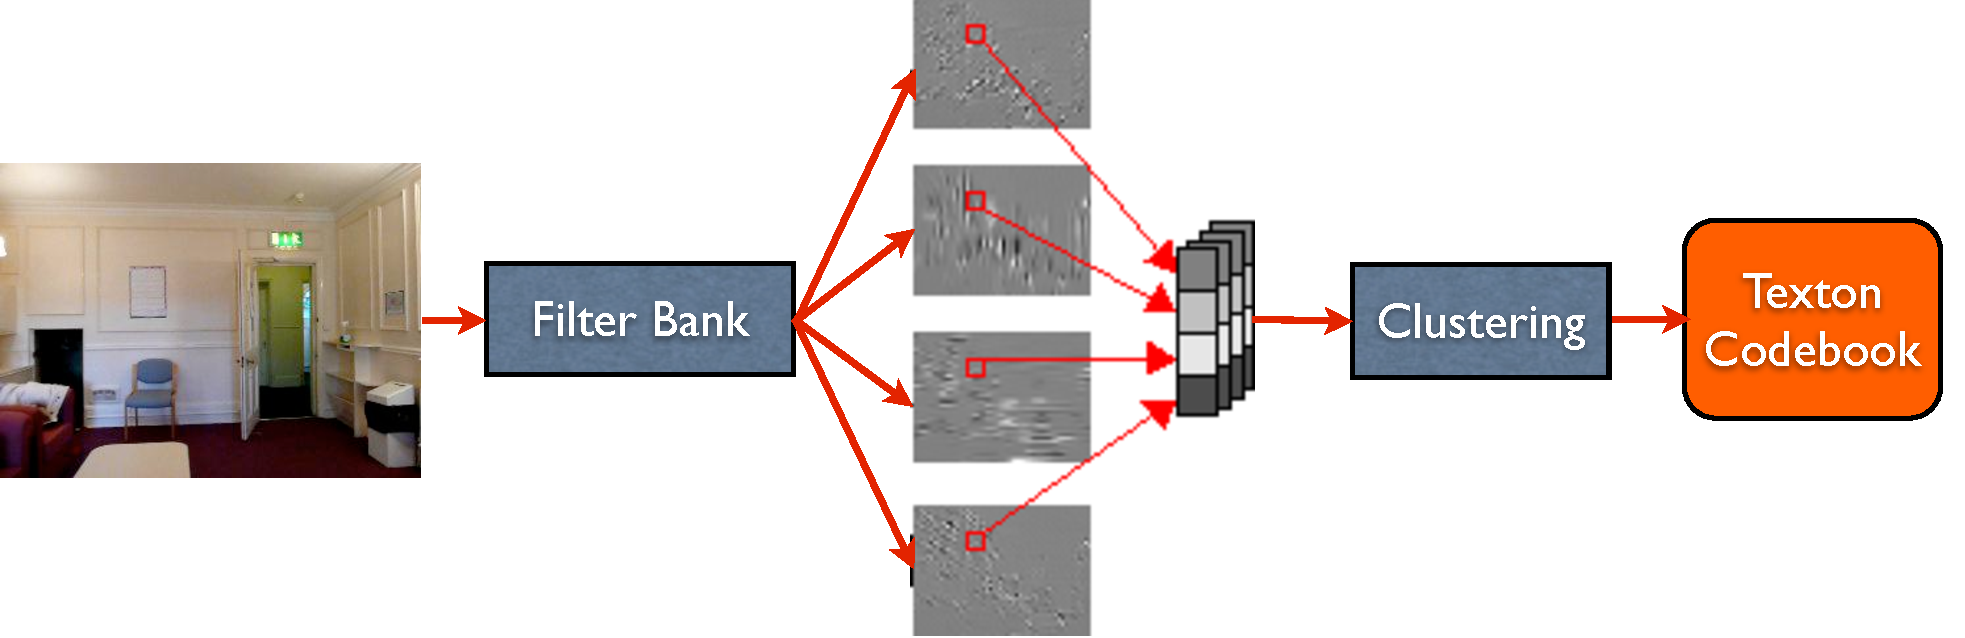
\includegraphics[width=\textwidth]{texton_process}
  \caption{The texton generation process.}
  \label{fig:texton-process}
\end{figure}

In the past textons have been successfully used to classify close--up
photos of materials such as wood, paper, and glass. Varma and
Zisserman \cite{Varma05} tackled this problem using the texton model
discussed above. After forming the texton map they proceed by counting
the occurrences of each texton, with the resultant histogram over
texton frequencies forming the model by which input images are matched
to their category. In their work, Varma and Zisserman apply a nearest
neighbour approach to classify the models, using the $\chi^2$
statistic to measure distances. Representing data by a histogram over
quantised features in this way has since become known by the
terminology ``bag--of--features'' or ``bag--of--words''.

\section{Textons for Scene Understanding}
Textons are a widely used and well--understood within the computer
vision community \cite{Zhu02,Varma05,Malik99}. However, their use has
mostly been limited to low--level image analysis tasks, such as
texture classification. We propose to use textons as the basis for
high--level reasoning tasks including scene classification. In the
remainder of this chapter we will develop a novel model by which to
utilise textons during inference. We begin in this section by
motivating the use of textons for this application.

Many place recognition systems rely upon an interest point detector
and descriptor to summarise input images
\cite{Fei-fei05,Cummins08}. This has proven effective for outdoor
environments as well as indoor environments that contain reasonably
distinctive landmarks. However, these systems are fundamentally
limited to a feature--centric view of the world in which only local
information about interest points is utilised.

We believe that there is un--leveraged information in the texture
structure within images, and that this can be used for scene
understanding tasks such as place recognition. Many images of indoor
scenes contain extremely poor visual information, particularly small,
empty environments like corridors and
foyers. \figref{low-saliency-frames} shows some examples of these. Yet
despite this information poverty, humans are capable of deducing much
from these images. For example, consider the image at the right of
\figref{low-saliency-frames}: there is barely one location here that
would yield a useful SIFT feature, yet a human can identify the part
of the environment that the image represents (a corner between wall
and ceiling), and a human familiar with the environment can easily
identify the room in which the image was captured. We think it is
clear that, in this case, humans are using a holistic understanding of
the image in which the edge structure together with the texture of the
surfaces is used to understand the image. We propose to use textons to
leverage this valuable information.

\begin{figure}[htp]
\centering
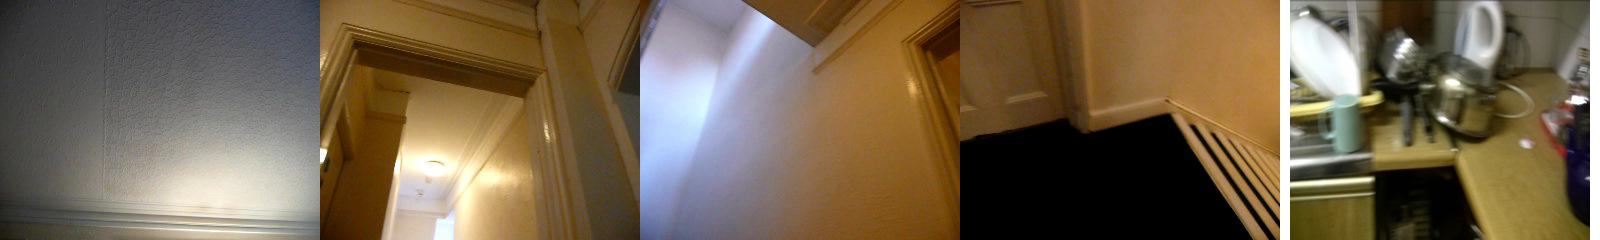
\includegraphics[width=\textwidth]{low_saliency.png}
\caption{Frames with low visual salience.}
\label{fig:low-saliency-frames}
\end{figure}

To investigate whether textons provide useful information about scene
structure, we collected video sequences of an indoor environment and
examined the textons generated by the algorithm described above. Our
dataset consisted of $10,555$ frames from $5$ rooms in a hostel. Some
qualitative findings are described in the following sections.

\subsection{Textons Select Salient Image Elements}
\figref{textons-generated} shows $25$ textons generated for this
dataset, in order of their frequency of occurrence. The first $7$
correspond to untextured regions of the image --- \ie
patches with near--uniform intensity. This is expected since the
majority of pixels lie within object or region boundaries, where
either the texture is too fine for the camera to detect (a carpet,
for example) or there simply is no texture (a white wall, for
example).

The next most frequent textons are those corresponding to edges and
bars at various orientations. Many image understanding algorithms
explicitly employ a line detector \cite{Forsyth02}, whereas in this
case the use of textons has allowed the system to learn to identify
these elements unsupervised.

At the other end of the frequency distribution, the least numerous
textons are those corresponding to image structures such as
junctions and line endpoints. These structures are also sought
explicitly in many image understanding algorithms \cite{Forsyth02},
whereas the use of textons selects these structures automatically and
unsupervised.

\begin{figure}[htp]
  \centering
  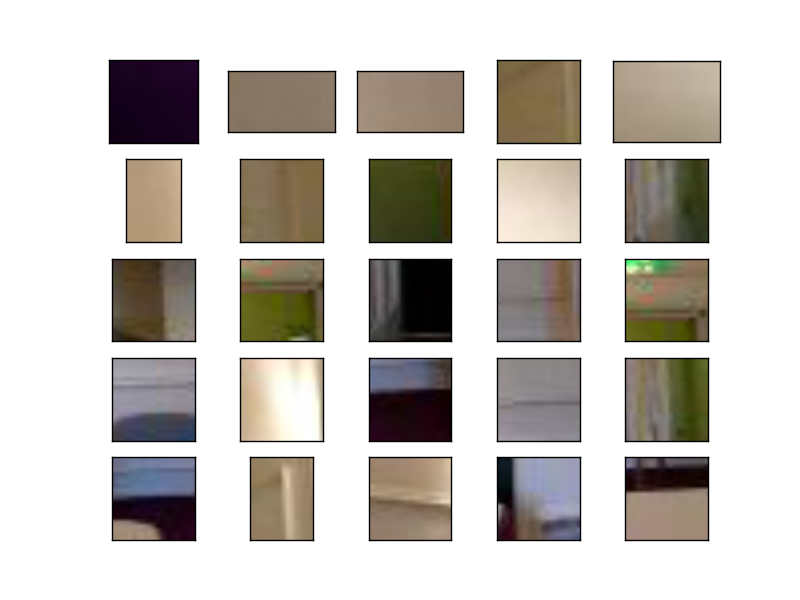
\includegraphics[width=\textwidth]{texton_exemplars}
  \caption{\changedsinceviva{
      Textons identified for our dataset during the offline
      training stage. Each panel shows a representative image patch for
      one of the cluster identified by K--means. The patches were
      selected by identifying the feature closest to each cluster
      centre, and then extracting a small patch about the image position
      from which it arose. The textons are sorted by
      decreasing frequency from top to bottom, left to right. Image
      patches are converted to grayscale before filtering, but here we
      show them in colour to assist visualisation. The patches vary in
      size due to clipping near image boundaries (this does not affect
      clustering).
    }
  }
  \label{fig:textons-generated}
\end{figure}

\subsection{Textons Focus Attention on Salient Image Regions}
\figref{texton-freq-distr} shows the frequency of each texton within
our entire dataset. The most frequent textons at the left of the graph
account for a disproportionately large number of pixels, whereas the
textons towards the right account for a tiny minority. We have just
seen that it is precisely these minority textons that correspond to
the image elements that are most useful in image understanding, so in
this sense the use of textons has automatically focused attention on
the small fraction of pixels representing the most salient image
structures.

\begin{figure}[htp]
  \centering
  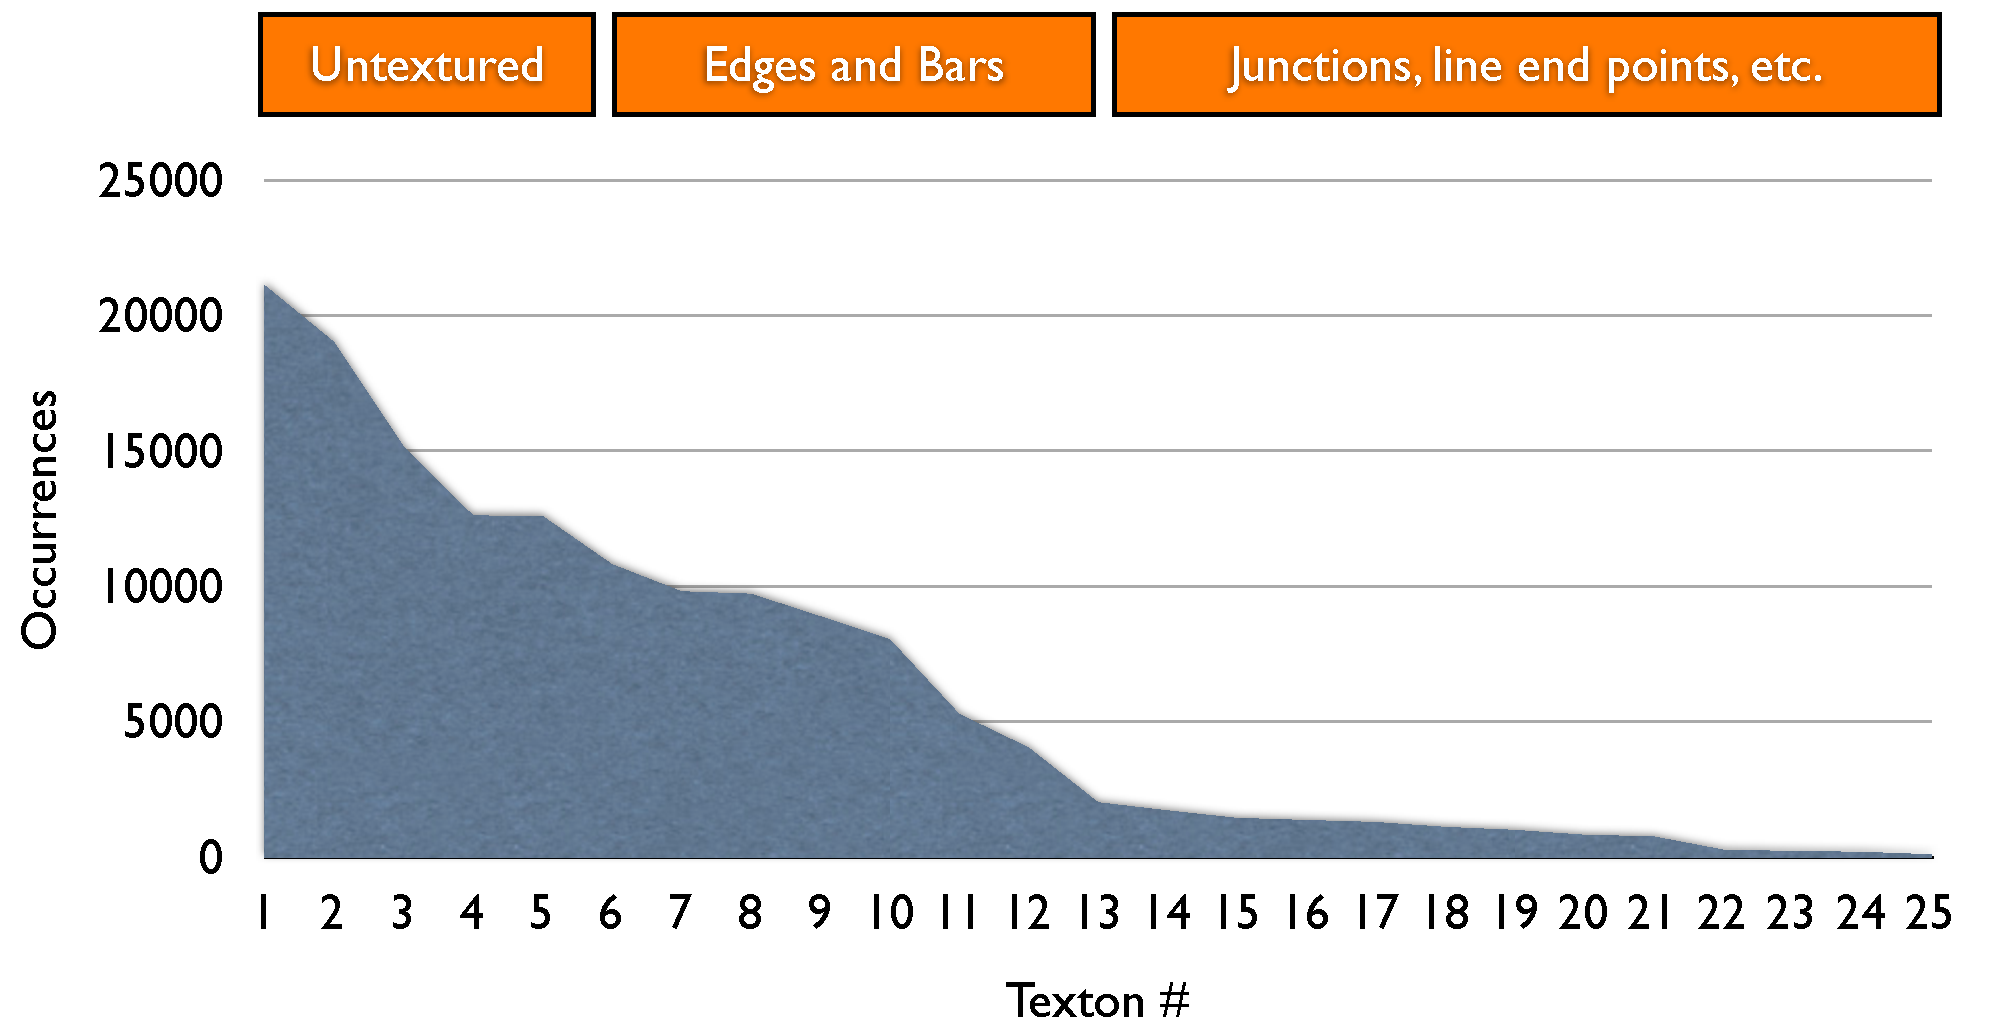
\includegraphics[width=0.8\textwidth]{texton_frequencies}
  \caption{Frequency distribution of textons. The texton generation
    process assigns more textons to describing salient but rare image
    structures such as junctions and line end points than it assigns to
    frequent but non--discriminative image regions such as textureless
    patches.}
  \label{fig:texton-freq-distr}
\end{figure}

\subsection{Textons Correlate With Scene Structure}
To further explore the relationship between textons and scene
structure we divided all frames within our dataset into three
orientation categories: ``straight'' (for which the camera's optical
axis was within $\pm 22.5\degrees$ of the horizontal), ``up'' (above
$22.5\degrees$), and ``down'' (below $22.5\degrees$). Next we computed
an average occupancy map for each texton within across each
category. Several per--texton heat--maps are shown in
\figref{eg-textons}. The first two rows show heat--maps for textons that
correspond roughly to ``floor'' and ``wall/ceiling''. We can see that
these reflect the image regions in which we would expect to find these
scene parts given the various camera orientations.

Perhaps the most instructive example of the texton/scene structure
relationship, however, is that of the textons that represent edge
elements, two of which are shown in the lower two rows of
\figref{eg-textons}. Consider the third row in this figure: The
stratification evident in the heat--map for downward--facing frames
indicates a common intersection somewhere above the image, whereas
that for the upward--facing frames indicates an intersection below the
image, and in the forward--facing frames the lines are close to
parallel. This, of course, is exactly what we would expect from our
understanding of projective camera geometry, but here our system has
automatically and without supervision captured these geometric
constraints (or at least some statistical form of them).

These illustration are simply indications that textons might provide
salient information of value for scene understanding. We describe our
model that explicitly relates these to each other in the next section.

\begin{figure*}[htp]
\centering
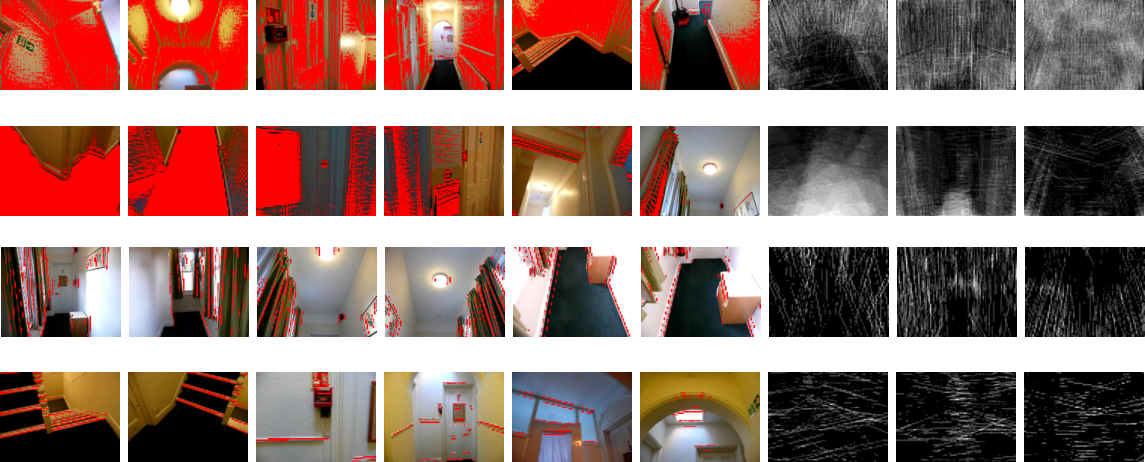
\includegraphics[width=\textwidth]{eg_textons.png}
\caption{Four example textons generated unsupervised for the camera
  orientation classification problem. From top to bottom the textons
  represent roughly ``wall or ceiling'', ``floor'', ``vertical edge'',
  and ``horizontal edge''. The six columns on the left show examples
  of where the texton was found. The three columns on the right show
  the average occupancy map over our dataset for images taken from an
  upwards--facing, horizontal, and downwards--facing camera (from left
  to right in the figure). The layout of the textons correlate
  strongly with camera orientation, which illustrates how our system
  is able to distinguish between camera orientations based on texton
  layout.}
\label{fig:eg-textons}
\end{figure*}

\section{Learning and Inference}
\label{sec:approach}
Having motivated the use of textons for image understanding we now
describe our probabilistic model that relates textons to scene
categories. For an input image $I$, we wish to discover the associated
place category $c$. For each category we are given a set of example
images at training time. We wish to model categories $c$ according
to the pixel locations in which textons appear within images
associated with each category. One popular approach is the
bag--of--features model \cite{Jebara03} but this would remove all
information about the locations of the textons, which as we have seen
is a principal source of salient information. Instead we propose a new
bag--of--texton--pairs model in which an image is represented as a
collection of observed texton pairs $\{(t_i, t_j, s_{i,j})\}$ where
$t_i$ and $t_j$ are texton labels and $s_{i,j}$ is the displacement
between the image locations at which they were observed. By
considering only displacements and not absolute pixel locations in our
model we gain some robustness to camera orientation.

For an image $I$ containing $N$ pixels there are $N^2$ such
pairwise observations. Our class--conditional likelihood is
\begin{equation}
P(I ~|~ c) = \prod_{i=0}^N \prod_{j=0}^N
P(t_i, ~ t_j, ~ s_{i,j} ~|~ c) \label{lik}
\end{equation}
where we have assumed independence between observations for
tractability. We compute the likelihood \eqref{lik} by estimating the
joint distribution $P(t_i,t_j,s_{i,j},c)$ using a histogram. We could
have used Parzen windowing \cite{Parzen62} for the continuous variable
$s_{i,j}$ but due to the very large number of samples we obtain for
each image, we found this to be unnecessary.

\changedsinceviva{
For images of reasonable size the cost of enumerating all $N^2$ texton
pairs is prohibitively expensive. We overcome this by overlaying an $M
\times M$ grid on the image and counting the occurrences of each
texton within each grid cell. We then enumerate all pairs of grid
cells and evaluate the texton pairs in aggregate. Hence for grid cells
$C_a$ and $C_b$ containing $n^a_i$ and $n^b_j$ instances of texton
$t_i$ and $t_j$ respectively, we evaluate $n^a_i n^b_j$ instances of
the observation $(t_i,t_j,s_{a,b})$ where $s_{a,b}$ is the distance
between the centres of the grid cells. We have lost some precision in
the texton locations since each texton is effectively moved to the
centre of the grid cell containing it, but our experiments show that
we are still able to capture sufficient salient information. We also
note that quantizing displacements in this way implicitly shares
information between similar displacements. One could think of this
operation as an efficient approximation to building the full joint
distribution and then smoothing along the displacement
axis.
}

During training we evaluate these aggregated observations by
multiplying the entry we make in the histogram by $n^a_i n^b_j$, and
during evaluation the aggregate observations correspond to
multiplications in the class--conditional log likelihood
\begin{eqnarray}
\log P(I ~|~ c) & = & \sum_{a=0}^{M^2} \sum_{b=0}^{M^2} \sum_{i=0}^K  \sum_{j=0}^K
 n^a_in^b_j \log P(t_i, ~ t_j, ~ s_{a,b} ~|~ c)
\end{eqnarray}
In both cases the aggregated observations can be evaluated in a single
step so the complexity is reduced from $O(N^2)$ to $O(M^4 K^2)$. In
practice we found that setting $M$$=$$8$, $K$$=$$25$ was sufficient to capture
much of the salient image information, while allowing our system to run
at video frame rate.

\section{Place Recognition}
\label{sec:place-recognition}
We applied our system to the problem of place recognition. Our data
set consisted of several video sequences captured in a hostel
using a low--quality camera with a resolution of $320 \times 240$,
which moved rapidly with the user's upper body. The sequences involved
frequent motion blur and rapid variations in camera orientation.

We labelled each frame with the place that it was captured in. There
were five labels: bedroom, kitchen, common room, garden, and
corridor. We gave all frames captured in corridors the same
label. This experiment does not correspond to place {\em category}
recognition since most of the labels included frames from only one
place instance. However, it is harder than strict landmark--style
localisation because, as shown in \figref{nonoverlapping}, many images
with the same label contain non--overlapping views of the room they
were captured in, yet the system is expected to recognise all of them
as belonging to the same place.

\begin{figure}[htp]
  \centering
  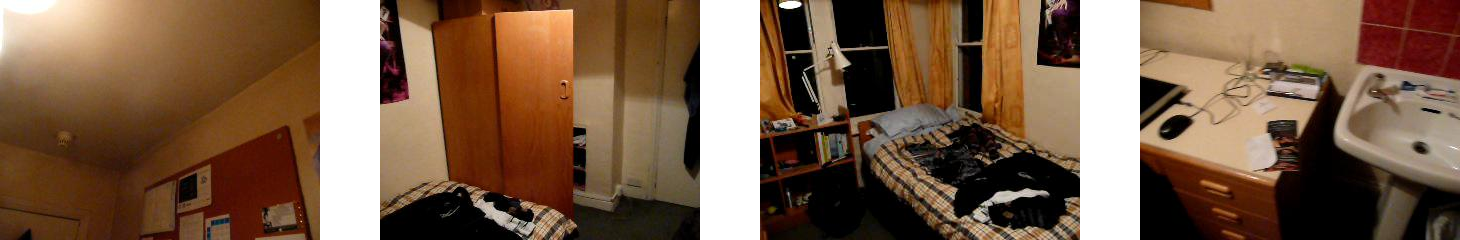
\includegraphics[width=\textwidth]{nonoverlapping.png}
  \caption{Four frames with the ``bedroom'' label. There are almost no
    overlapping scene parts but the system is required to (and did
    successfully) recognise each of them as part of the same place.}
  \label{fig:nonoverlapping}
\end{figure}

We compared our system with the gist descriptor of Torralba \etal and
a K--nearest--neighbours baseline, using vectorised grayscale images
as feature vectors for the latter. For the gist descriptor we used the
same Gabor filter bank that we used in our own system and we estimated
the class--conditional likelihood in feature space by building
Gaussian mixture models with the Gaussians constrained to be
spherical, exactly as described in \cite{Torralba03}.

Initially we used 230 frames for training and 490 frames for
evaluation (our training and evaluation sets were taken from separate
sequences). The results from this experiment are shown in the middle
row of \tableref{place-cla-results} and in
\figref{place-confusion}. Our system outperformed Torralba's by a
large margin. We suspected that the poor performance of Torralba's
system was due to the training data not sufficiently populating the
32--dimensional feature space. This exemplifies one of the major
advantages of our approach: the ability to learn from limited training
data. However, to show that this is not the \textit{only} advantage of
our approach we ran auxiliary experiments with larger and smaller
training sets. When the training set was enlarged our system
outperformed Torralba's by a significant but smaller margin, and when
the training set was decreased, the performance of our system
decreased only slightly whereas Torralba's system was unable to
estimate the Gaussian mixture due to the sparsity of training
samples. The latter case corresponds to just 20 examples per
label. These results are shown in the top and bottom rows of
\tableref{place-cla-results}.

Figures \ref{fig:pos-examples} and \ref{fig:neg-examples} show
positive and negative results from our system. Note how our system
recognises images containing disjoint views of a room as belonging to
the same place.

\begin{table}[htb]
  \centering
  \begin{tabular}{@{}p{40mm}p{30mm}p{30mm}p{40mm}@{}}
    \toprule
      No. training frames &
      This chapter &
      Torralba \etal &
      Nearest neighbours \\
    \midrule
      103 & \textbf{81\%} & --- & 45\% \\
      230 & \textbf{83\%} & 62\% & 52\% \\
      565 & \textbf{85\%} & 70\% & 55\% \\
    \bottomrule
  \end{tabular}
  \caption{Recognition rate for the place recognition problem with
    varying numbers of training examples. The reported accuracy is the
    mean over the on--diagonal elements of the confusion matrix. The
    left column reports the total number of training examples for all
    categories. For the experiment with 103 training examples we were
    unable to estimate the Gaussian mixtures required for the system
    of Torralba \etal due to the sparsity of the training
    examples. The nearest neighbours baseline was computed by resizing
    images to 64 by 64 pixels and comparing raw pixel intensities in
    the L2 sense.}
  \label{table:place-cla-results}
\end{table}

\begin{figure}[htp]
  \centering
  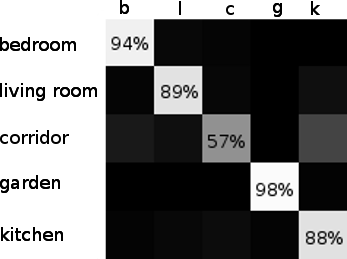
\includegraphics[width=0.4\textwidth]{place_confusion}
  \caption{Confusion matrix for place recognition. This figure
    corresponds to the bottom row of \tableref{place-cla-results}.}
  \label{fig:place-confusion}
\end{figure}

\begin{figure*}[htp]
\centering
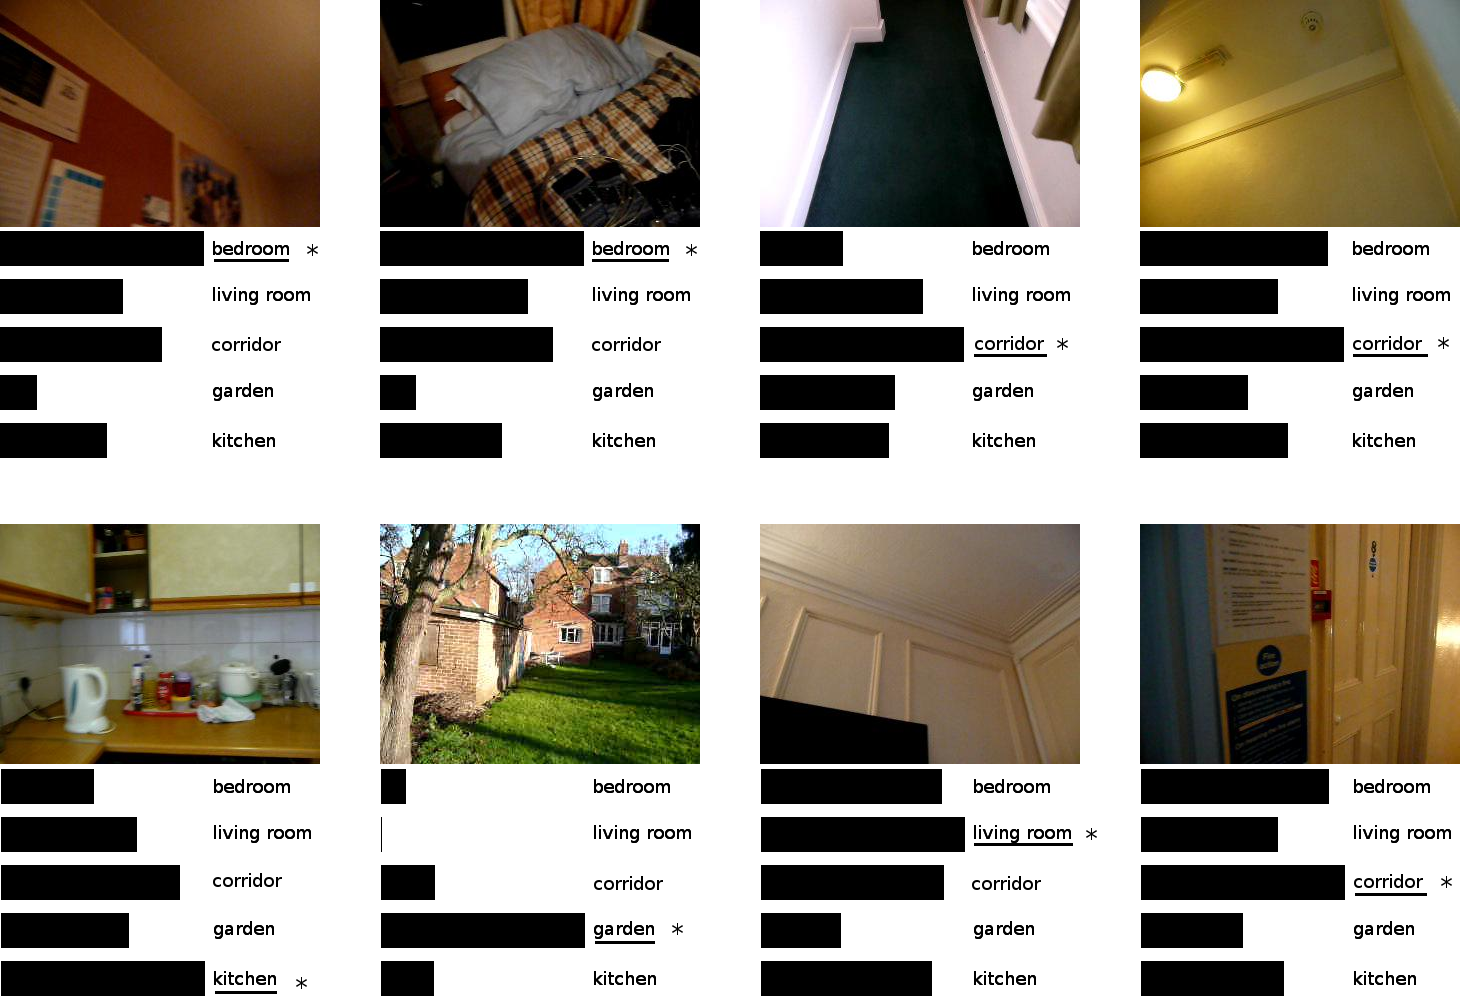
\includegraphics[width=\textwidth]{pos_examples.png}
\caption{Example frames for which our classifier produced the correct
  output. The ground truth label is underlined and the output from our
  system is starred. We show the posterior distribution over class
  labels in black. Note the variation between images with the same
  label, and the low quality of many images.}
\label{fig:pos-examples}
\end{figure*}

\begin{figure*}[htp]
\centering
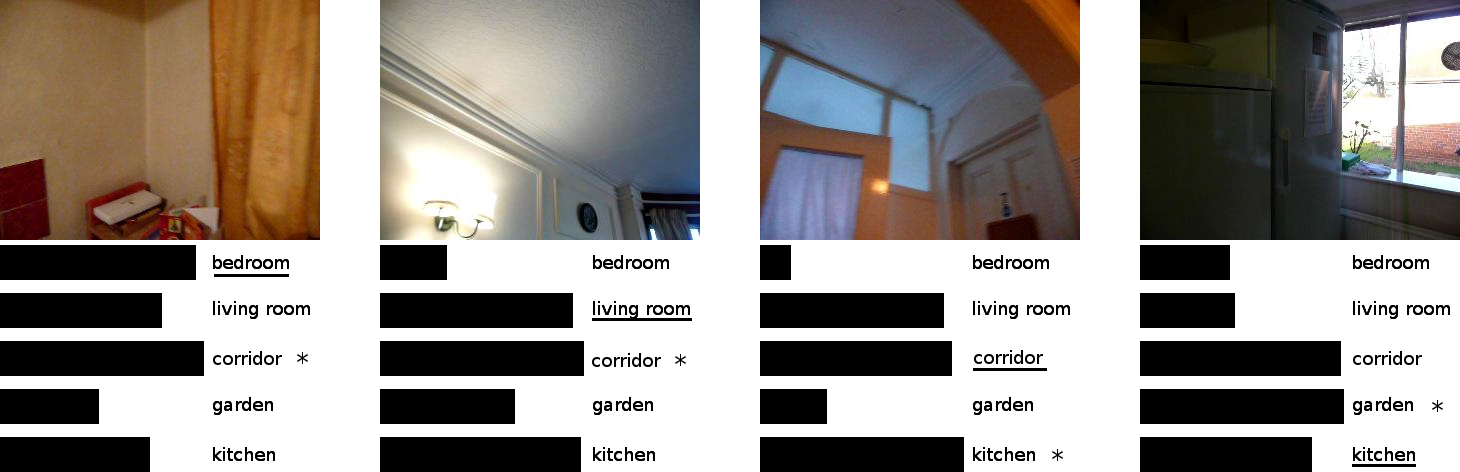
\includegraphics[width=\textwidth]{neg_examples.png}
\caption{Example frames for which our classifier failed. See caption
  of \figref{pos-examples}.}
\label{fig:neg-examples}
\end{figure*}

\section{Camera Orientation Classification}
\label{sec:camera-orientation}
In this section we show how our system can deduce a coarse camera
orientation from a single image. We are interested only in the tilt of
the camera with respect to the ground plane. Our intention is to make
a rapid but coarse estimate of camera orientation. We pose the problem
as a classification task with three labels: ``up'', ``straight'', and
``down''. The ``straight'' label represents images taken with the
camera axis parallel to the ground plane, plus or minus
$22.5^{\circ}$, and the ``up'' and ``down'' labels represent all
orientations facing further upwards or downwards respectively (see
\figref{camorients}).

\begin{figure}[htp]
  \centering
  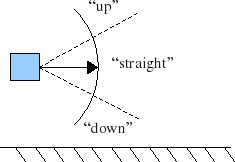
\includegraphics[width=0.4\textwidth]{camorients}
  \caption{Definition of the labels for camera orientation recognition.}
  \label{fig:camorients}
\end{figure}

We captured three sequences in which the camera orientation was fixed
within one of the above orientation ranges. We included footage from
five different places (the same rooms used in the previous section) but
we labelled the frames according to orientation only. This represents
a difficult classification task because the system must learn
properties that correlate with camera orientation but are not tied to
the appearance of a particular room. We then trained our system to
distinguish between the three orientation categories as in the
previous section.

We again compared with the ``gist'' of Torralba {\em et al.} and a KNN
baseline. We ran auxiliary experiments with an enlarged training set
as in the previous section. The results of these experiments are shown
in \tableref{orient-cla-results} and \figref{orient-confusion}. Our
system again outperformed both other classifiers by a significant
margin. Some example frames for which our system correctly identified
the camera orientation are shown in \figref{eg-orients}. Of particular
interest is our system's ability to generalise across images taken
with the same camera orientation at several different locations.

\begin{table}[htb]
  \centering
  \begin{tabular}{@{}p{40mm}p{30mm}p{30mm}p{40mm}@{}}
    \toprule
      No. training frames &
      This chapter &
      Torralba \etal &
      Nearest neighbours \\
    \midrule
      88 & \textbf{70\%} & 61\% & 59\% \\
      728 & \textbf{79\%} & 63\% & 59\% \\
    \bottomrule
  \end{tabular}
    \caption{Camera orientation classification results using small and
      large training sets. The reported accuracies are the average of
      the on--diagonal entries in the confusion matrix. In this case
      we were able to estimate the Gaussians for Torralba's system
      using only 88 training examples because there were fewer categories
      than in the place recognition problem. The nearest neighbours
      baseline was computed by resizing images to 64 by 64
      pixels and comparing raw pixel intensities in the L2 sense.}
  \label{table:orient-cla-results}
\end{table}

\begin{figure}[htp]
  \centering
  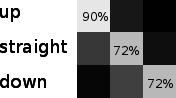
\includegraphics[width=0.25\textwidth]{orient_confusion}
  \caption{Confusion matrix for camera orientation
    classification. This figure shows results corresponding to the
    bottom row in \tableref{orient-cla-results}.}
  \label{fig:orient-confusion}
\end{figure}

\begin{figure}[htp]
\centering
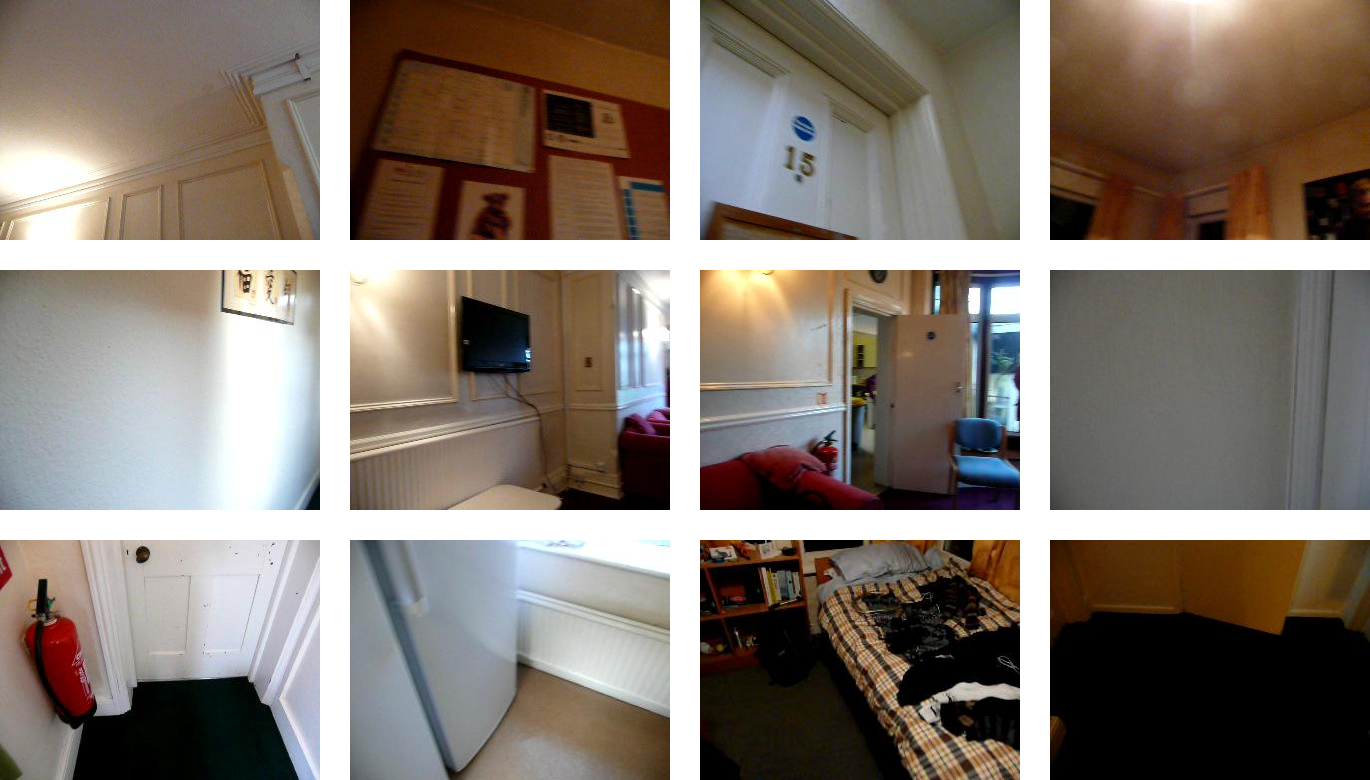
\includegraphics[width=\textwidth]{orient_egs.png}
\caption{Twelve frames for which our system correctly identified the
  camera orientation. From the top to bottom the rows contain images
  from the ``up'', ``straight'', and ``down'' classes.}
\label{fig:eg-orients}
\end{figure}


\section{Computational Concerns}
The most computationally demanding aspect of our system is the
convolutions needed to generate the pixel features. In this section we
describe several optimisations for the convolution operation. Timing
results are shown in \tableref{convolve-timing} at the end of this
section.

\subsection{Separable Kernels}
The Gabor function, which we use to generate pixel features, in its
canonical form is a complex--valued function and can be trivially
separated. However, in our work we use just the real part,
\begin{eqnarray}
  H_{real}(x,y) & = & g_2(x,y) \cos(kx\cos\theta + ky\sin\theta) ~,
\end{eqnarray}
where $g_2$ is the two--dimensional Gaussian
function. This can be written as the difference between two separable
function as
\begin{eqnarray}
  %H_{real}(x,y) & = & g_2(x,y) \cos(ax + by)\\
  %  & = & g_1(x)g_1(y) \Bigl(\cos ax\cos (by) - \sin ax \sin by
  %    \Bigr) \label{sep2}\\
   H_{real}(x,y) & = & \Bigl(g_1(x)\cos ax\Bigr) \Bigl(g_1(y)\cos by\Bigr)
      - \Bigl(g_1(x)\sin ax\Bigr)\Bigl(g_1(y)\sin by\Bigr)
\end{eqnarray}
where $g_1$ is the one--dimensional Gaussian function and we have used
the cosine expansion formula. We implement this by running two
separated convolutions and then taking their difference, which is
significantly faster than performing the original convolution.

\subsection{Parallelization over filters}
Generating the pixel features requires convolving an input image with
12 different filters. To leverage the parallelism of
modern multi--core CPUs we execute the convolutions in parallel where
possible. This approach allows parallelization within a single scale,
but requires synchronisation upon completion of each scale due to the
down--sampling operation.

\subsection{Parallelization over pixels}
Modern graphics hardware allows efficient parallelization of
small--scale computations such as per--pixel operations. This is is
well suited to performing convolutions since each output pixel is
functionally independent of all others. To leverage this we
implemented convolutions using a C--like language designed
specifically for programming graphics hardware. We note that further
improvements may be possible since under the current implementation,
much time is spent transferring data between the CPU and GPU, in
comparison to which the time spent performing the convolutions is
small. This bottleneck could be partially avoided if we performed the
texton labelling in the GPU and transferred only the final texton map
back to the CPU.

\subsection{Timing results}
Results from timing evaluations are shown in
\tableref{convolve-timing}. The GPU strategy outperforms all
others. It improves over the baseline strategy by a factor of $5$ for
the $320 \times 240$ image and by a factor of $6$ for the $640 \times
480$ image.


It is interesting to note \changedsinceviva{that when} the image is
enlarged to include four times as many pixels, the three CPU--based
strategies degrade by a factor very close to four, whereas the GPU
implementation degrades by a factor closer to three. This indicates
that this task saturates CPU performance but that a significant
overhead remains in the GPU implementation. This matches our
observation in the previous section that transmitting data between the
CPU and GPU consumes much time, and that further performance
improvements are possible.



\begin{table}[htp]
  \centering
  \begin{tabular}{@{}p{40mm}p{20mm}p{20mm}p{20mm}p{20mm}@{}}
    \toprule
      & \multicolumn{2}{c}{\textbf{320 $\times$ 240}}
      & \multicolumn{2}{c}{\textbf{640 $\times$ 480}} \\
      \textbf{Strategy} &
      \textbf{Per Frame} &
      \textbf{Frame Rate} &
      \textbf{Per Frame} &
      \textbf{Frame Rate} \\
    \midrule
      No parallelization & 115.0ms & 8.69Hz & 463.6ms & 2.16Hz \\
      Filter--parallel & 38.0ms & 26.3Hz & 148.0ms & 6.76Hz \\
      Image--parallel & 32.1ms & 31.2Hz & 125.6ms & 8.02Hz \\
      Pixel--parallel (GPU) & 23.5ms & 42.5Hz & 78.1ms & 12.80Hz \\
    \bottomrule
  \end{tabular}
  \caption{Timing results for the four parallelization strategies. Each
    strategy was evaluated for two image sizes. All strategies utilise
    separated filters. Results are averages over 10 invocations.}
  \label{table:convolve-timing}
\end{table}

\section{Conclusions}
In this chapter we have shown that texture structure can be leveraged
to deduce high--level information about image scenes. We have
motivated the use of textons for this purpose with several qualitative
examples, and have presented results from two in--depth
experiments. In both cases our system based on relative displacements
between textons obtains highly encouraging results. Furthermore, by
utilising graphics hardware our system is capable of operating at
video frame rate.

%% We also note an intruiging line of investigation in which we could
%% treat the labelling process as a classification task with the values
%% from a neighbourhood about a pixel as inputs and the texton labels as
%% output. Since the filters only use local information anyway, it seems
%% possible to build an accurate classifier to operate on raw pixel
%% values, which would avoid both the convolution and nearest--neighbour
%% matching steps. The challenge, of course, would be to build a
%% classifier fast enough that this substitution resulted in a beneficial
%% trade--off. Perhaps randomized forrests would be suitable here. We
%% intend to pursue this line of investigation only if it is necessary
%% to achieve real--time performance.

%% \section{Choice of Filter Banks}

%% The use of filter banks in computer vision long pre--dates the texton
%% literature. A wide variety of kernel functions have been proposed such
%% as difference-- and derivative--of--Gaussians (¬cite), wavelets (Gabor
%% filter are particularly popular ¬cite), steerable pyramids
%% \cite{Freeman91}, and many others. Motivations for choosing one kernel
%% over another include expressiveness, orthogonality, efficiency,
%% simplicity, invariance to image transformations such as rotations
%% (¬cite), and the ability to reconstruct the original image from its
%% filtered form.

%% Our experience indicates that, among those kernel functions in
%% widespread use today, our system is largely unaffected by the specific
%% kernel chosen. That is not to say that the choice of kernel function
%% is unimportant \textit{per se}, but rather that, for our purposes, many
%% modern kernel functions provide equal amounts of salient information
%% from which our system is capable of learning. We chose the Gabor
%% kernel because of its theoretical basis in wavelet theory, its
%% simplicity of implementation, and its separability.

%% Varma and Zisserman \cite{Varma03} have suggested that filter banks
%% may not be necessary for texture classification at all. They
%% demonstrate that filter banks can be replaced by simply using the
%% values in a 9--neighbourhood about each pixel as that pixel's feature
%% vector, in which case their texture classifier performs equally as
%% well as when filter banks are used. We have not investigated whether
%% such a strategy would is suitable for our task. We intend to
%% experiment with this idea because from an efficiency point of view
%% avoiding the need for the convolution step entirely is attractive.
